\documentclass{article}
\usepackage[utf8]{inputenc}
\usepackage{graphicx}
\usepackage{hyperref}
\usepackage[margin=1in]{geometry}

\title{Supplementary Material:\\Tail Heaviness Controls Explosive Synchronization}
\author{DataLab-atom Collaboration}
\date{}

\begin{document}
\maketitle

This supplement provides 29 additional figures supporting the main text.

\section{Benchmark and Classical Verification}

\begin{figure}[h]\centering

\includegraphics[width=0.7\textwidth]{supplementary/benchmark_classical.pdf}
\caption{Classical Kuramoto benchmark: $r$ vs $K_2$ with theoretical $K_c=1.596$ line and $\sqrt{K_2-K_c}$ scaling verification.}
\end{figure}

\begin{figure}[h]\centering

\includegraphics[width=0.7\textwidth]{supplementary/oa_verification.pdf}
\caption{OA $K_c$ accuracy: comparison of old vs corrected $\Delta$ formula vs numerical.}
\end{figure}

\section{Phase Diagrams}

\begin{figure}[h]\centering

\includegraphics[width=\textwidth]{supplementary/fig1_phase_diagram_matrix.pdf}
\caption{Full $K_2\times K_3$ phase diagram matrix across six $\sigma$ values.}
\end{figure}

\begin{figure}[h]\centering
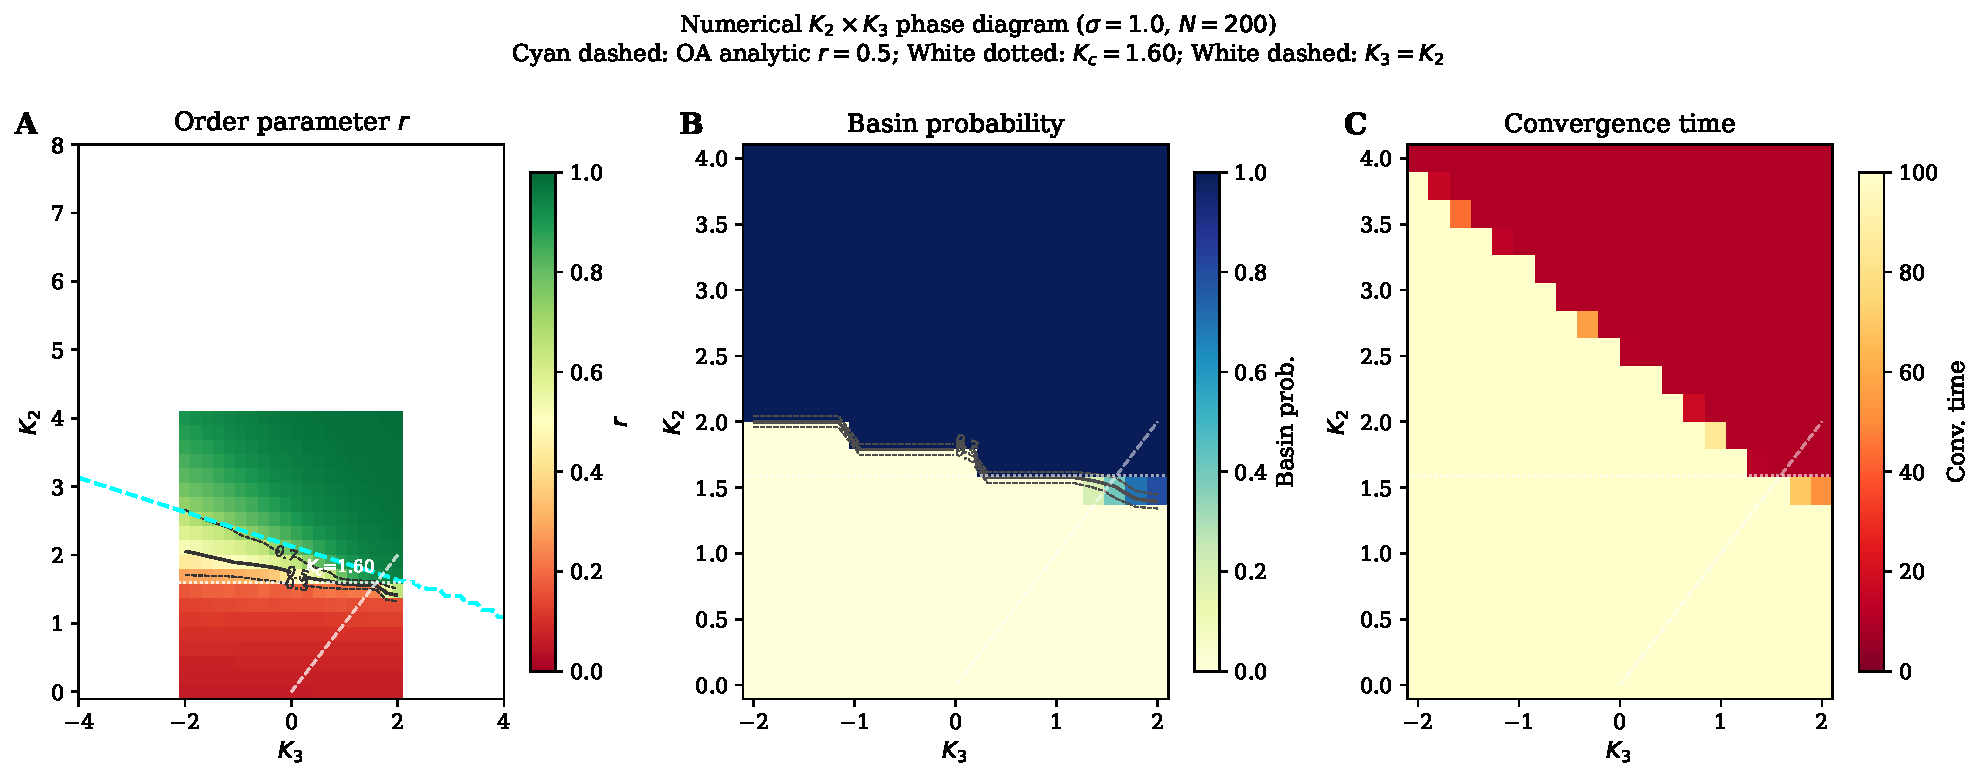
\includegraphics[width=0.7\textwidth]{supplementary/numerical_phase_K2K3.pdf}
\caption{Numerical $K_2\times K_3$ phase diagram ($N=200$, $\sigma=1$).}
\end{figure}

\begin{figure}[h]\centering

\includegraphics[width=\textwidth]{supplementary/analytic_phase_diagrams.pdf}
\caption{Analytic phase diagrams from OA reduction for six $\sigma$ values.}
\end{figure}

\begin{figure}[h]\centering

\includegraphics[width=0.7\textwidth]{supplementary/corrected_vs_numerical.pdf}
\caption{Corrected self-consistent equation vs numerical: side-by-side comparison showing $<3\%$ error for $\sigma\le1.0$.}
\end{figure}

\section{$\sigma$ and Distribution Effects}

\begin{figure}[h]\centering
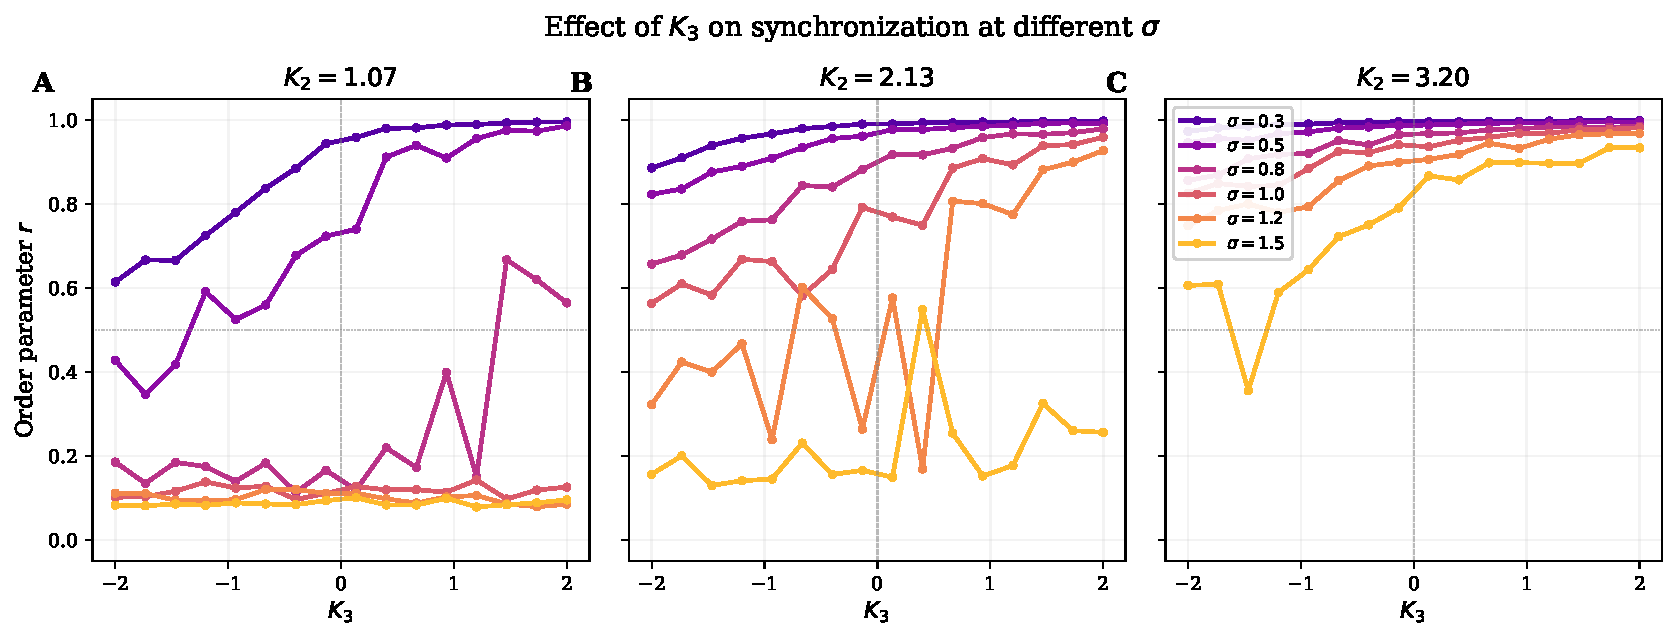
\includegraphics[width=\textwidth]{supplementary/fig2_sigma_effect.pdf}
\caption{$\sigma$ effect curves at three $K_2$ cross-sections.}
\end{figure}

\begin{figure}[h]\centering

\includegraphics[width=0.7\textwidth]{supplementary/fig3_Kc_shift.pdf}
\caption{$K_c$ shift for five $K_3$ values vs corrected theoretical predictions.}
\end{figure}

\begin{figure}[h]\centering
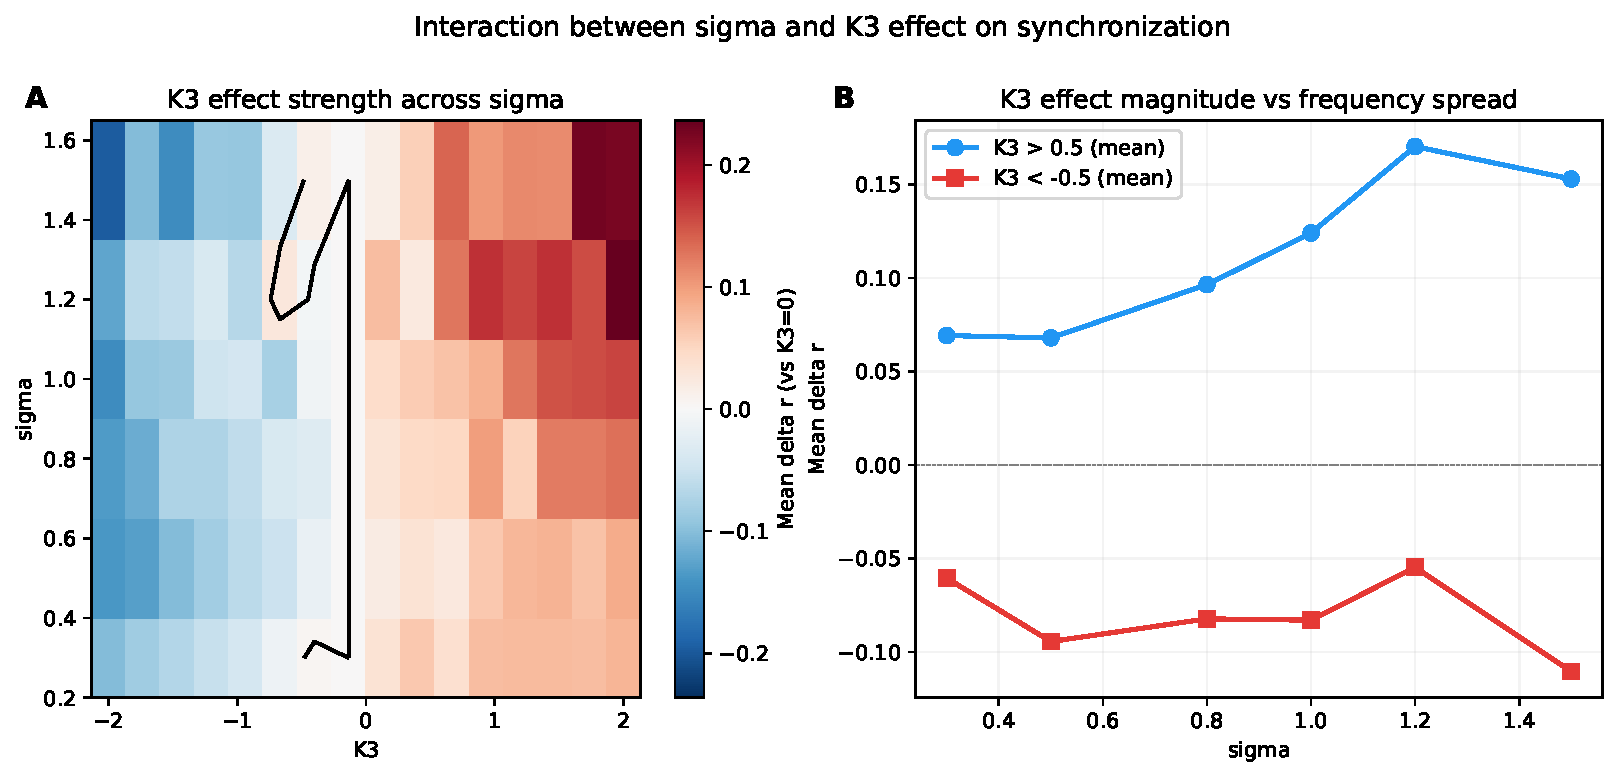
\includegraphics[width=0.7\textwidth]{supplementary/sigma_K3_interaction.pdf}
\caption{$\sigma\times K_3$ interaction: $K_3$ effect strength varies with $\sigma$.}
\end{figure}

\begin{figure}[h]\centering

\includegraphics[width=0.7\textwidth]{supplementary/freq_distribution.pdf}
\caption{Frequency distribution comparison: Gaussian, Lorentzian, Uniform. $K_3>0$ helps in all three.}
\end{figure}

\begin{figure}[h]\centering

\includegraphics[width=0.7\textwidth]{supplementary/gaussian_exact.pdf}
\caption{Gaussian exact self-consistent equation vs Lorentzian OA comparison.}
\end{figure}

\begin{figure}[h]\centering
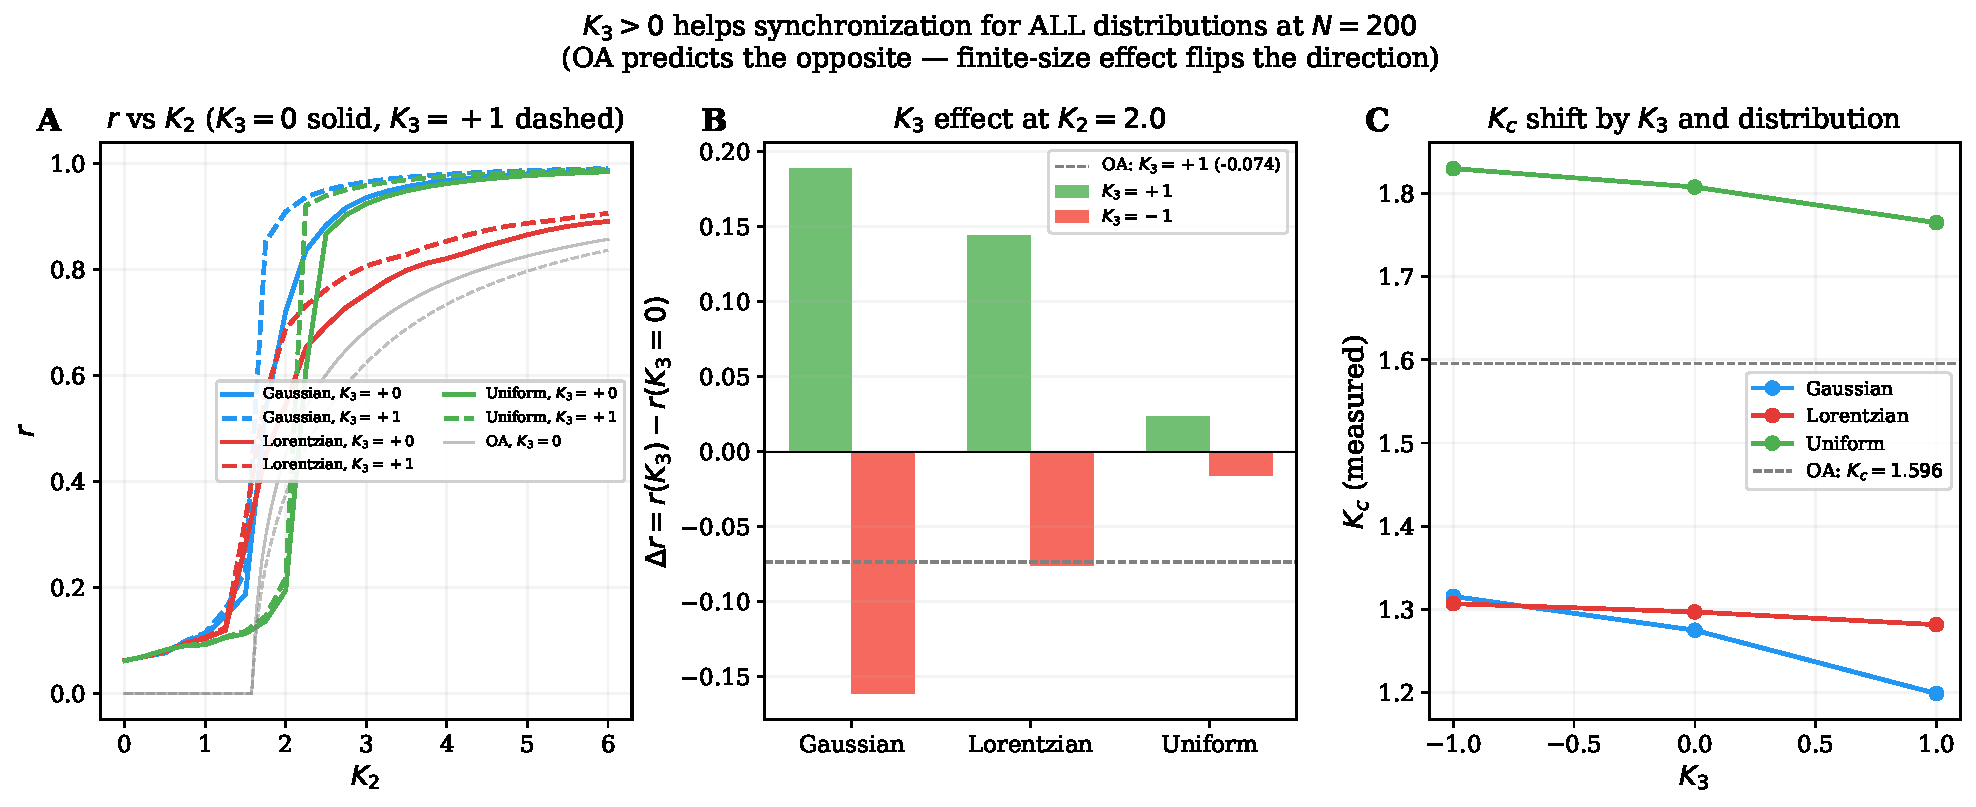
\includegraphics[width=0.7\textwidth]{supplementary/dist_K3_direction.pdf}
\caption{$K_3$ effect direction across distributions: all show enhancement at $N=200$.}
\end{figure}

\section{Metrics and Stability}

\begin{figure}[h]\centering

\includegraphics[width=\textwidth]{supplementary/fig4_triple_metric.pdf}
\caption{Three synchronization metrics ($r$, basin probability, convergence time) jointly.}
\end{figure}

\begin{figure}[h]\centering

\includegraphics[width=0.7\textwidth]{supplementary/fig5_basin_vs_stability.pdf}
\caption{Basin probability vs stability depth scatter.}
\end{figure}

\begin{figure}[h]\centering

\includegraphics[width=0.7\textwidth]{supplementary/Kc_vs_K3.pdf}
\caption{Effective $K_c$ vs $K_3$: onset remains constant, saddle-node shifts.}
\end{figure}

\section{$K_3$ Asymmetry and Locking}

\begin{figure}[h]\centering
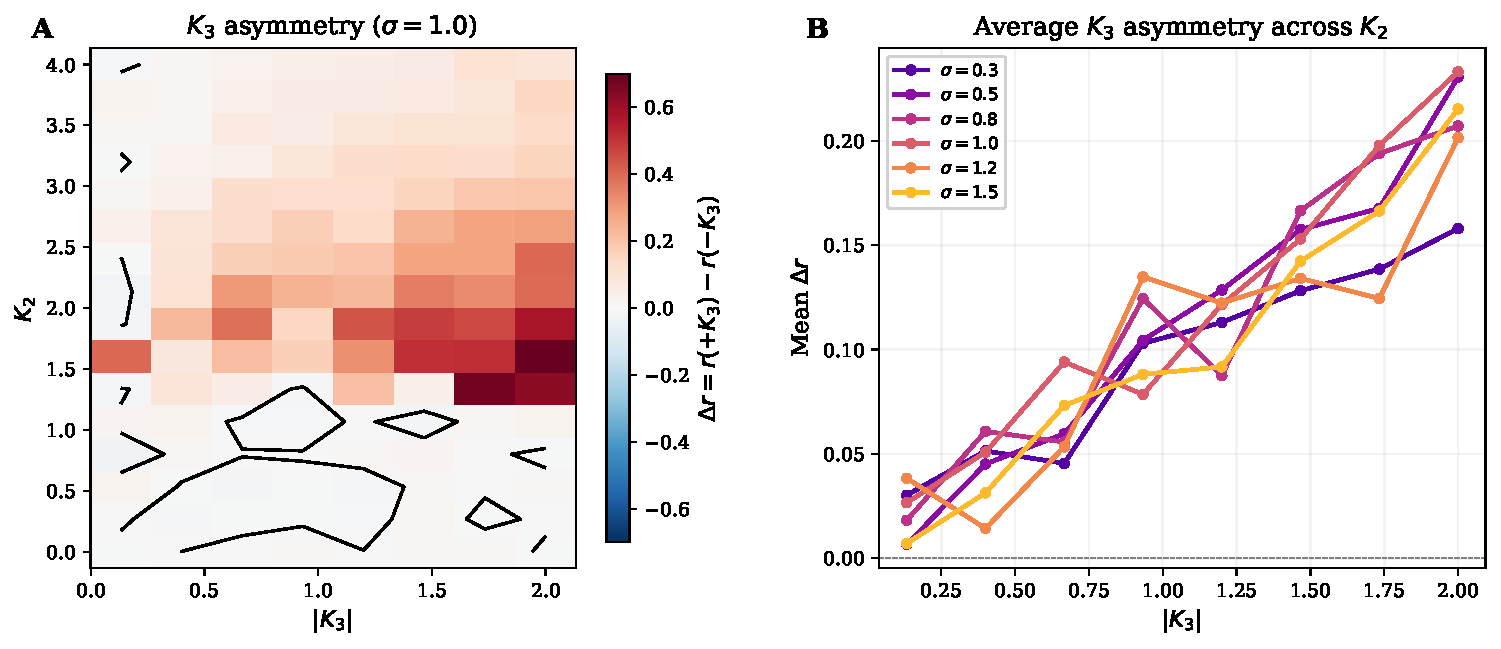
\includegraphics[width=\textwidth]{supplementary/fig6_asymmetry.pdf}
\caption{Extended $K_3$ asymmetry analysis.}
\end{figure}

\begin{figure}[h]\centering
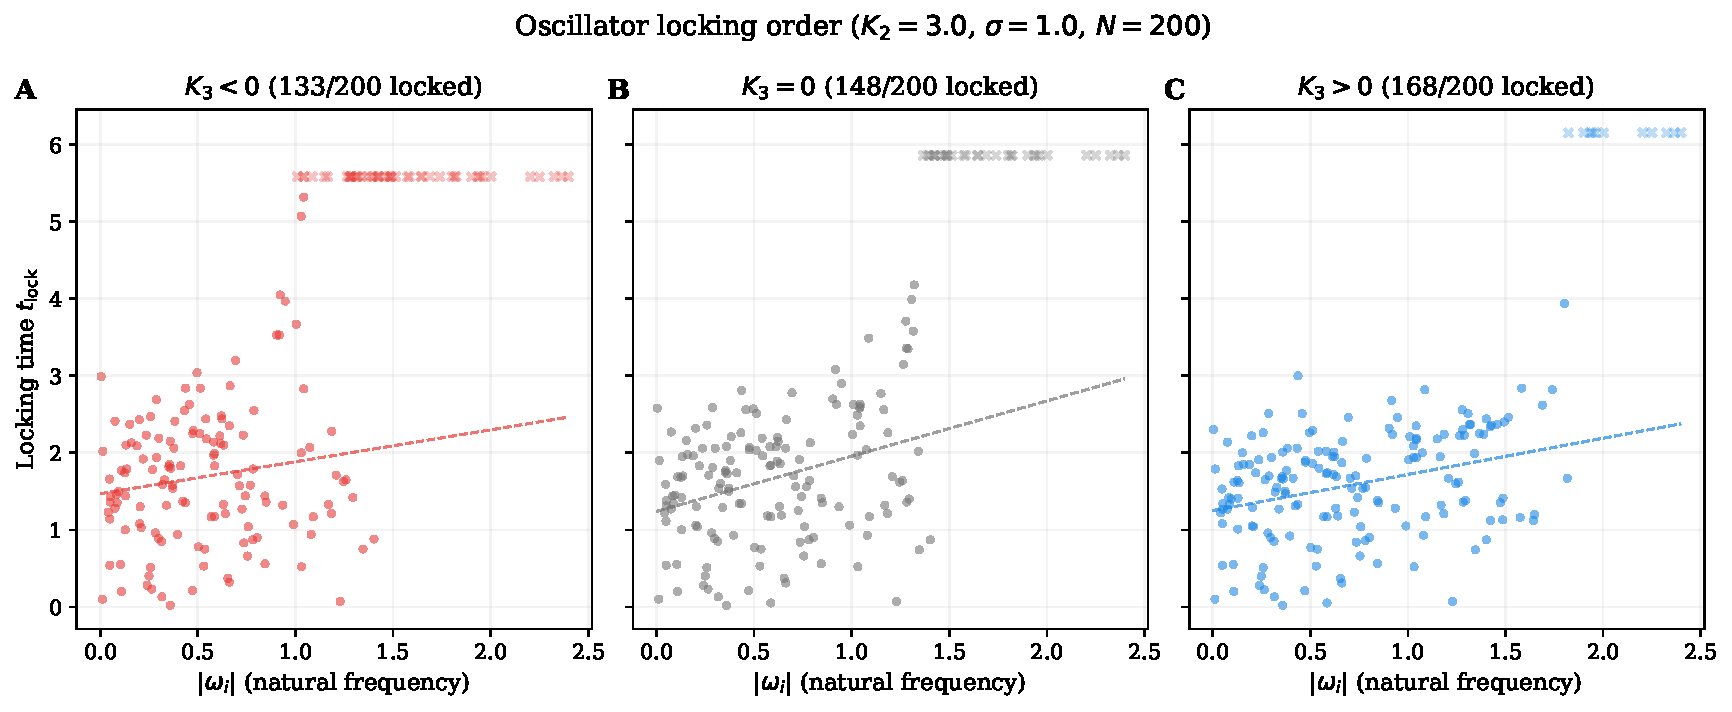
\includegraphics[width=0.7\textwidth]{supplementary/locking_order.pdf}
\caption{Locking order: $t_{\mathrm{lock}}$ vs $|\omega_i|$ scatter for three $K_3$ values.}
\end{figure}

\begin{figure}[h]\centering

\includegraphics[width=0.7\textwidth]{supplementary/K3_help_hurt_map.pdf}
\caption{Map of where $K_3>0$ helps vs hurts: 97\% help, 3\% exceptions near $K_c$.}
\end{figure}

\section{Hysteresis and Transitions}

\begin{figure}[h]\centering
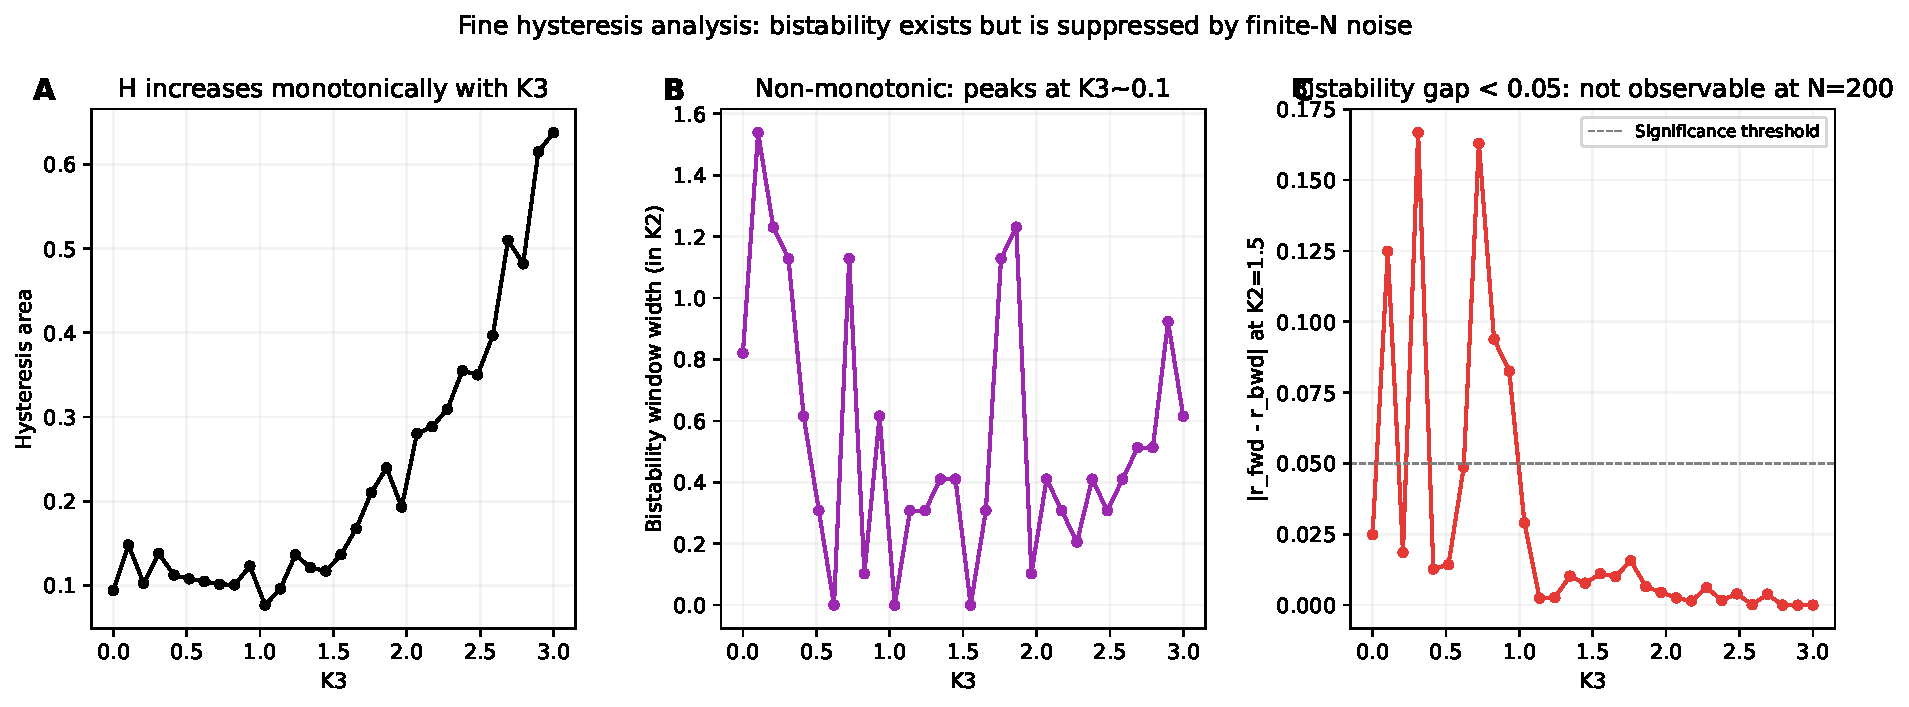
\includegraphics[width=\textwidth]{supplementary/hysteresis_fine.pdf}
\caption{Fine-grained hysteresis: 30 $K_3$ values, area non-monotonic with minimum at $K_3\approx1.0$.}
\end{figure}

\begin{figure}[h]\centering
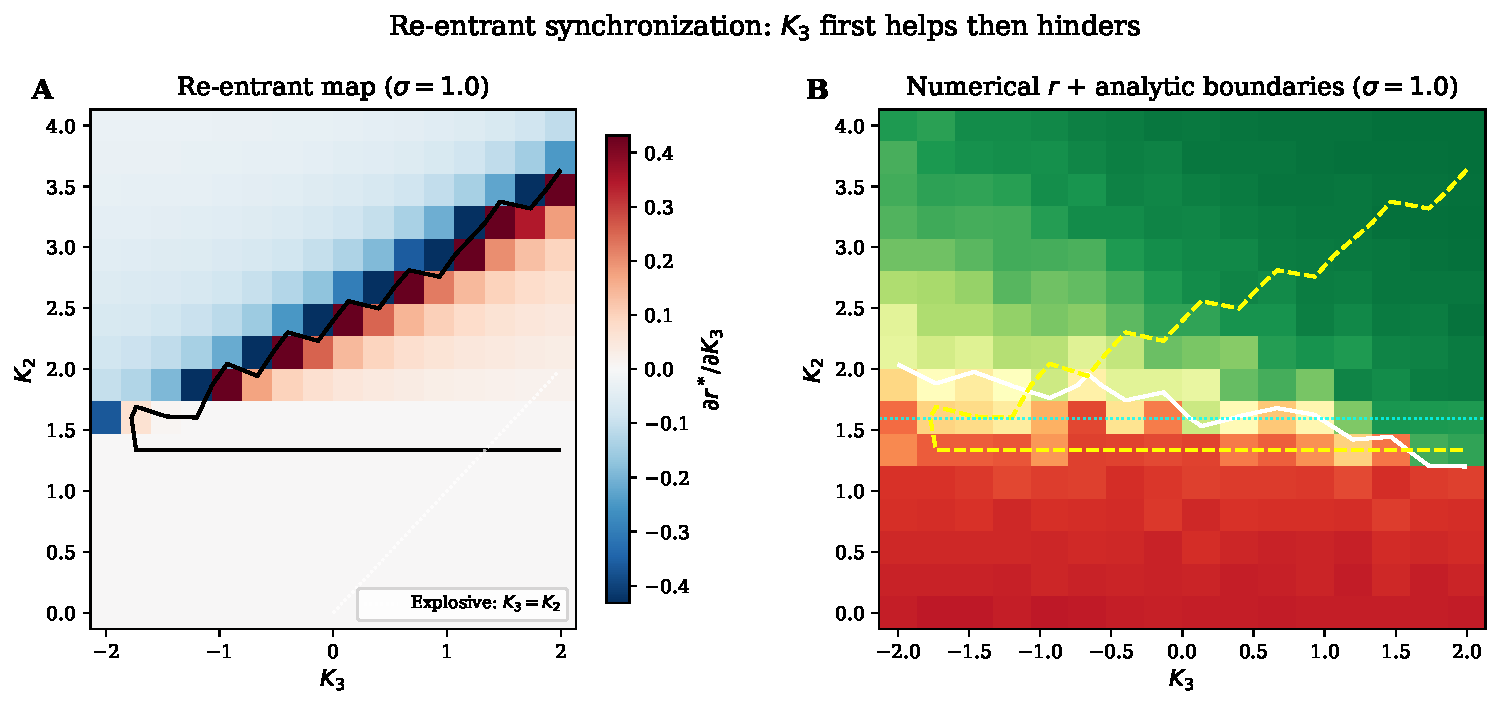
\includegraphics[width=0.7\textwidth]{supplementary/fig8_reentrant.pdf}
\caption{$\partial r^*/\partial K_3$ map: no re-entrant region detected (monotonic increase everywhere).}
\end{figure}

\section{OA Validity and Corrections}

\begin{figure}[h]\centering
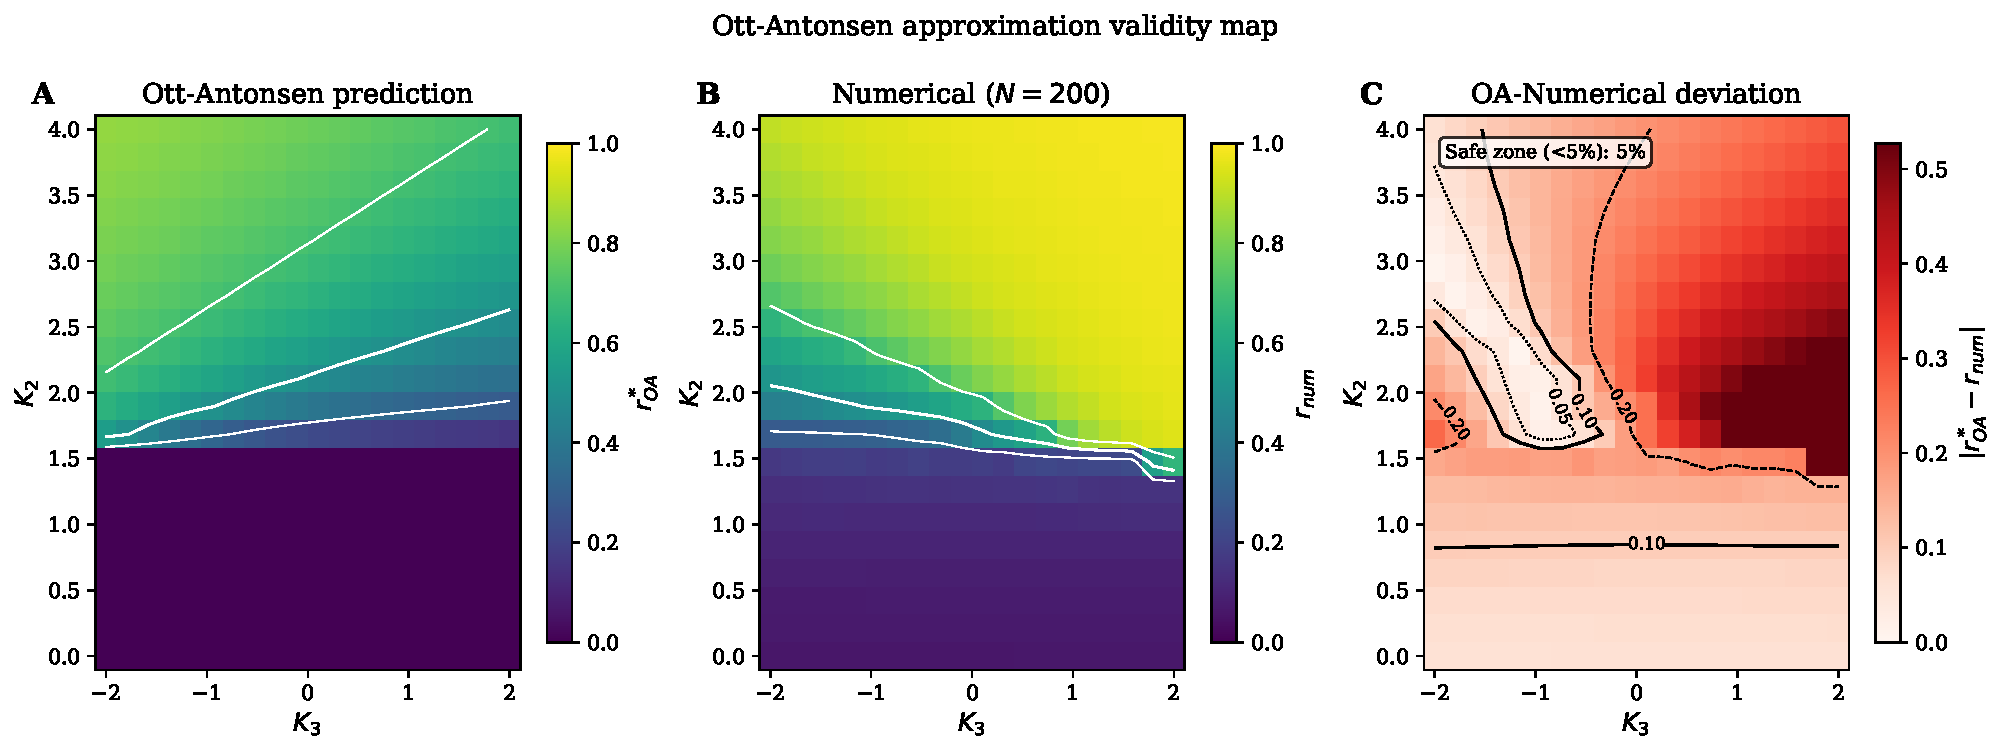
\includegraphics[width=0.7\textwidth]{supplementary/oa_deviation.pdf}
\caption{OA deviation heatmap: $|r^*_{\mathrm{OA}}-r_{\mathrm{num}}|$ across $K_2\times K_3$.}
\end{figure}

\begin{figure}[h]\centering

\includegraphics[width=0.7\textwidth]{supplementary/fig7_analytic_vs_numeric.pdf}
\caption{Analytic vs numeric $r$ comparison (original OA).}
\end{figure}

\begin{figure}[h]\centering
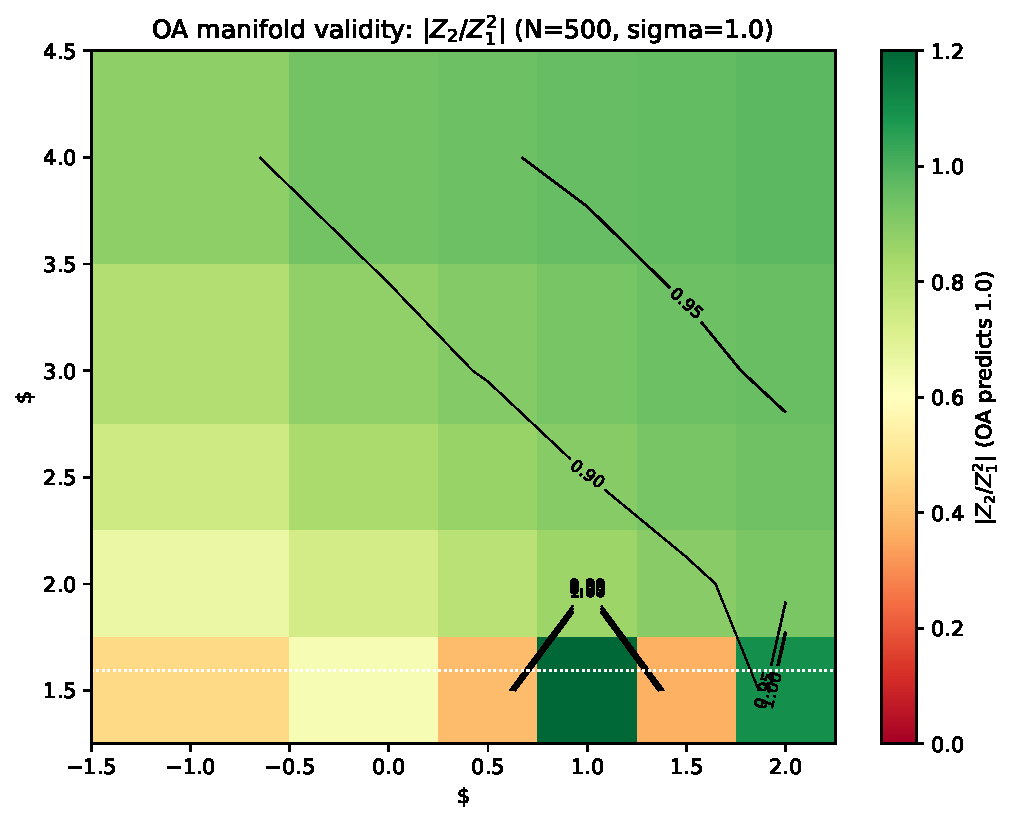
\includegraphics[width=0.7\textwidth]{supplementary/Z2_Z1_ratio.pdf}
\caption{$Z_2/Z_1^2$ ratio: deviates from OA prediction ($=1$) at negative $K_3$.}
\end{figure}

\section{Higher-Order and Structural Effects}

\begin{figure}[h]\centering

\includegraphics[width=0.7\textwidth]{supplementary/K4_effect.pdf}
\caption{Four-body coupling $K_4$ effect: non-negligible at $N=50$ (89\% of $K_3$), decreasing with $N$.}
\end{figure}

\begin{figure}[h]\centering
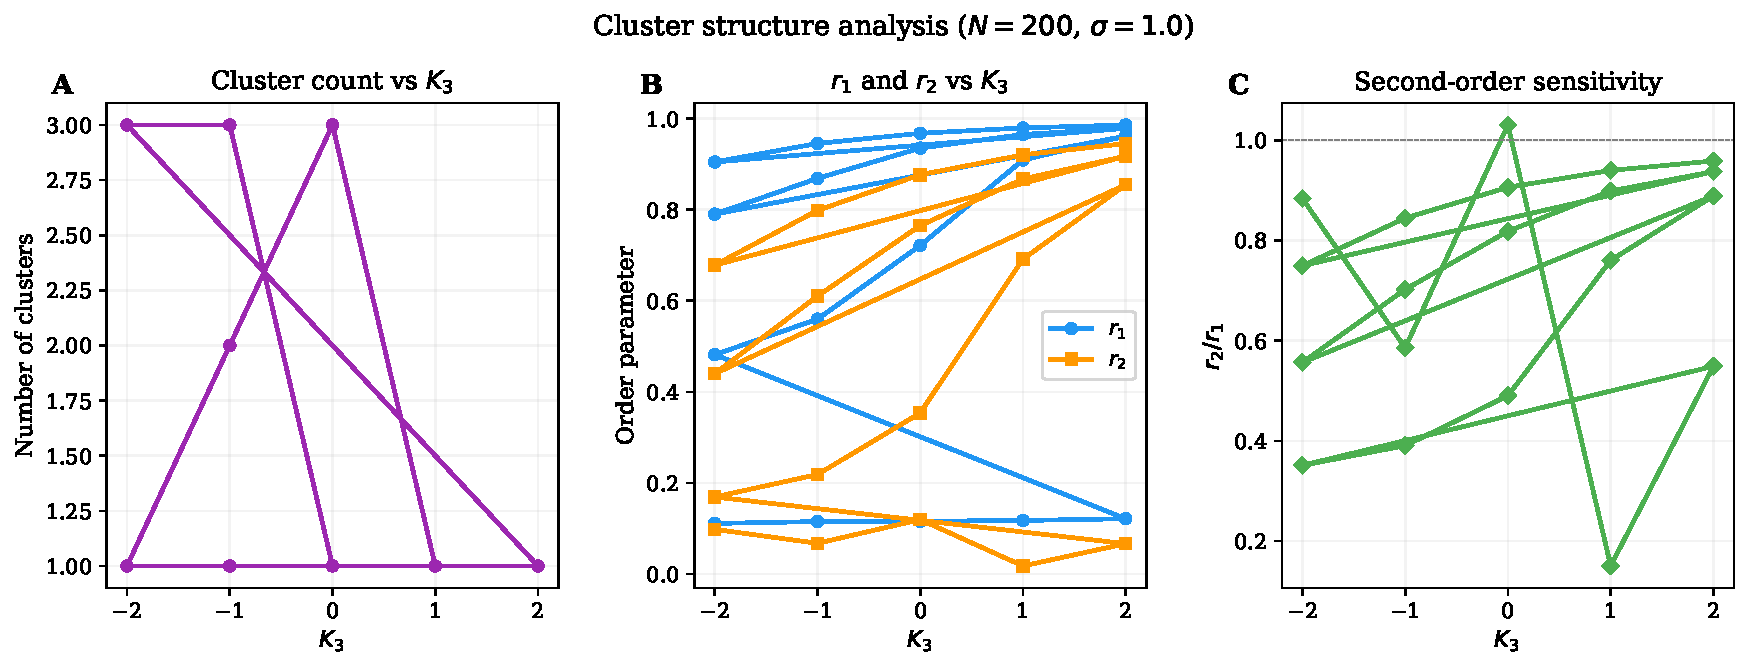
\includegraphics[width=0.7\textwidth]{supplementary/cluster_structure.pdf}
\caption{Cluster structure: multi-cluster (2--3) appears only at $K_3<0$ in frustration zone.}
\end{figure}

\begin{figure}[h]\centering
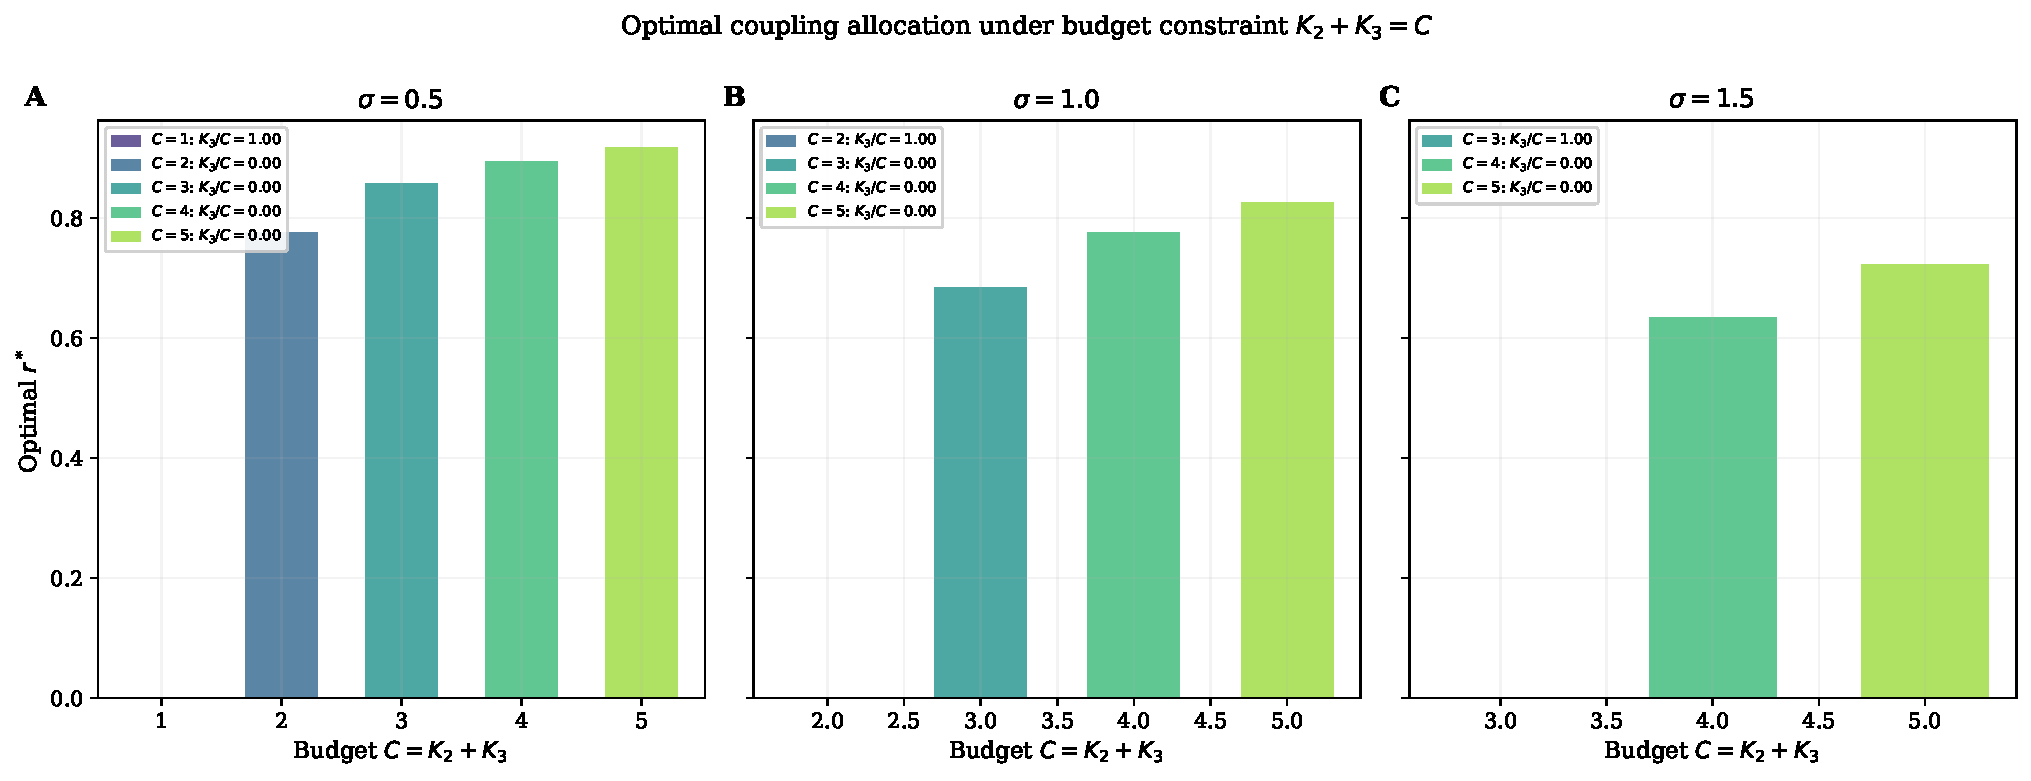
\includegraphics[width=0.7\textwidth]{supplementary/budget_optimization.pdf}
\caption{Budget-constrained optimization: pure pairwise ($K_3=0$) always optimal on all-to-all networks.}
\end{figure}

\section{Finite-Size Effects}

\begin{figure}[h]\centering

\includegraphics[width=0.7\textwidth]{supplementary/finite_size_K3.pdf}
\caption{Finite-size $K_3$ effect: $\Delta r$ increases from $N=20$ to $N=500$.}
\end{figure}

\begin{figure}[h]\centering

\includegraphics[width=0.7\textwidth]{supplementary/finite_size_large_N.pdf}
\caption{Large-$N$ convergence: $N=200$ to $N=20000$, approaching Gaussian exact prediction.}
\end{figure}

\section{Summary}

\begin{figure}[h]\centering
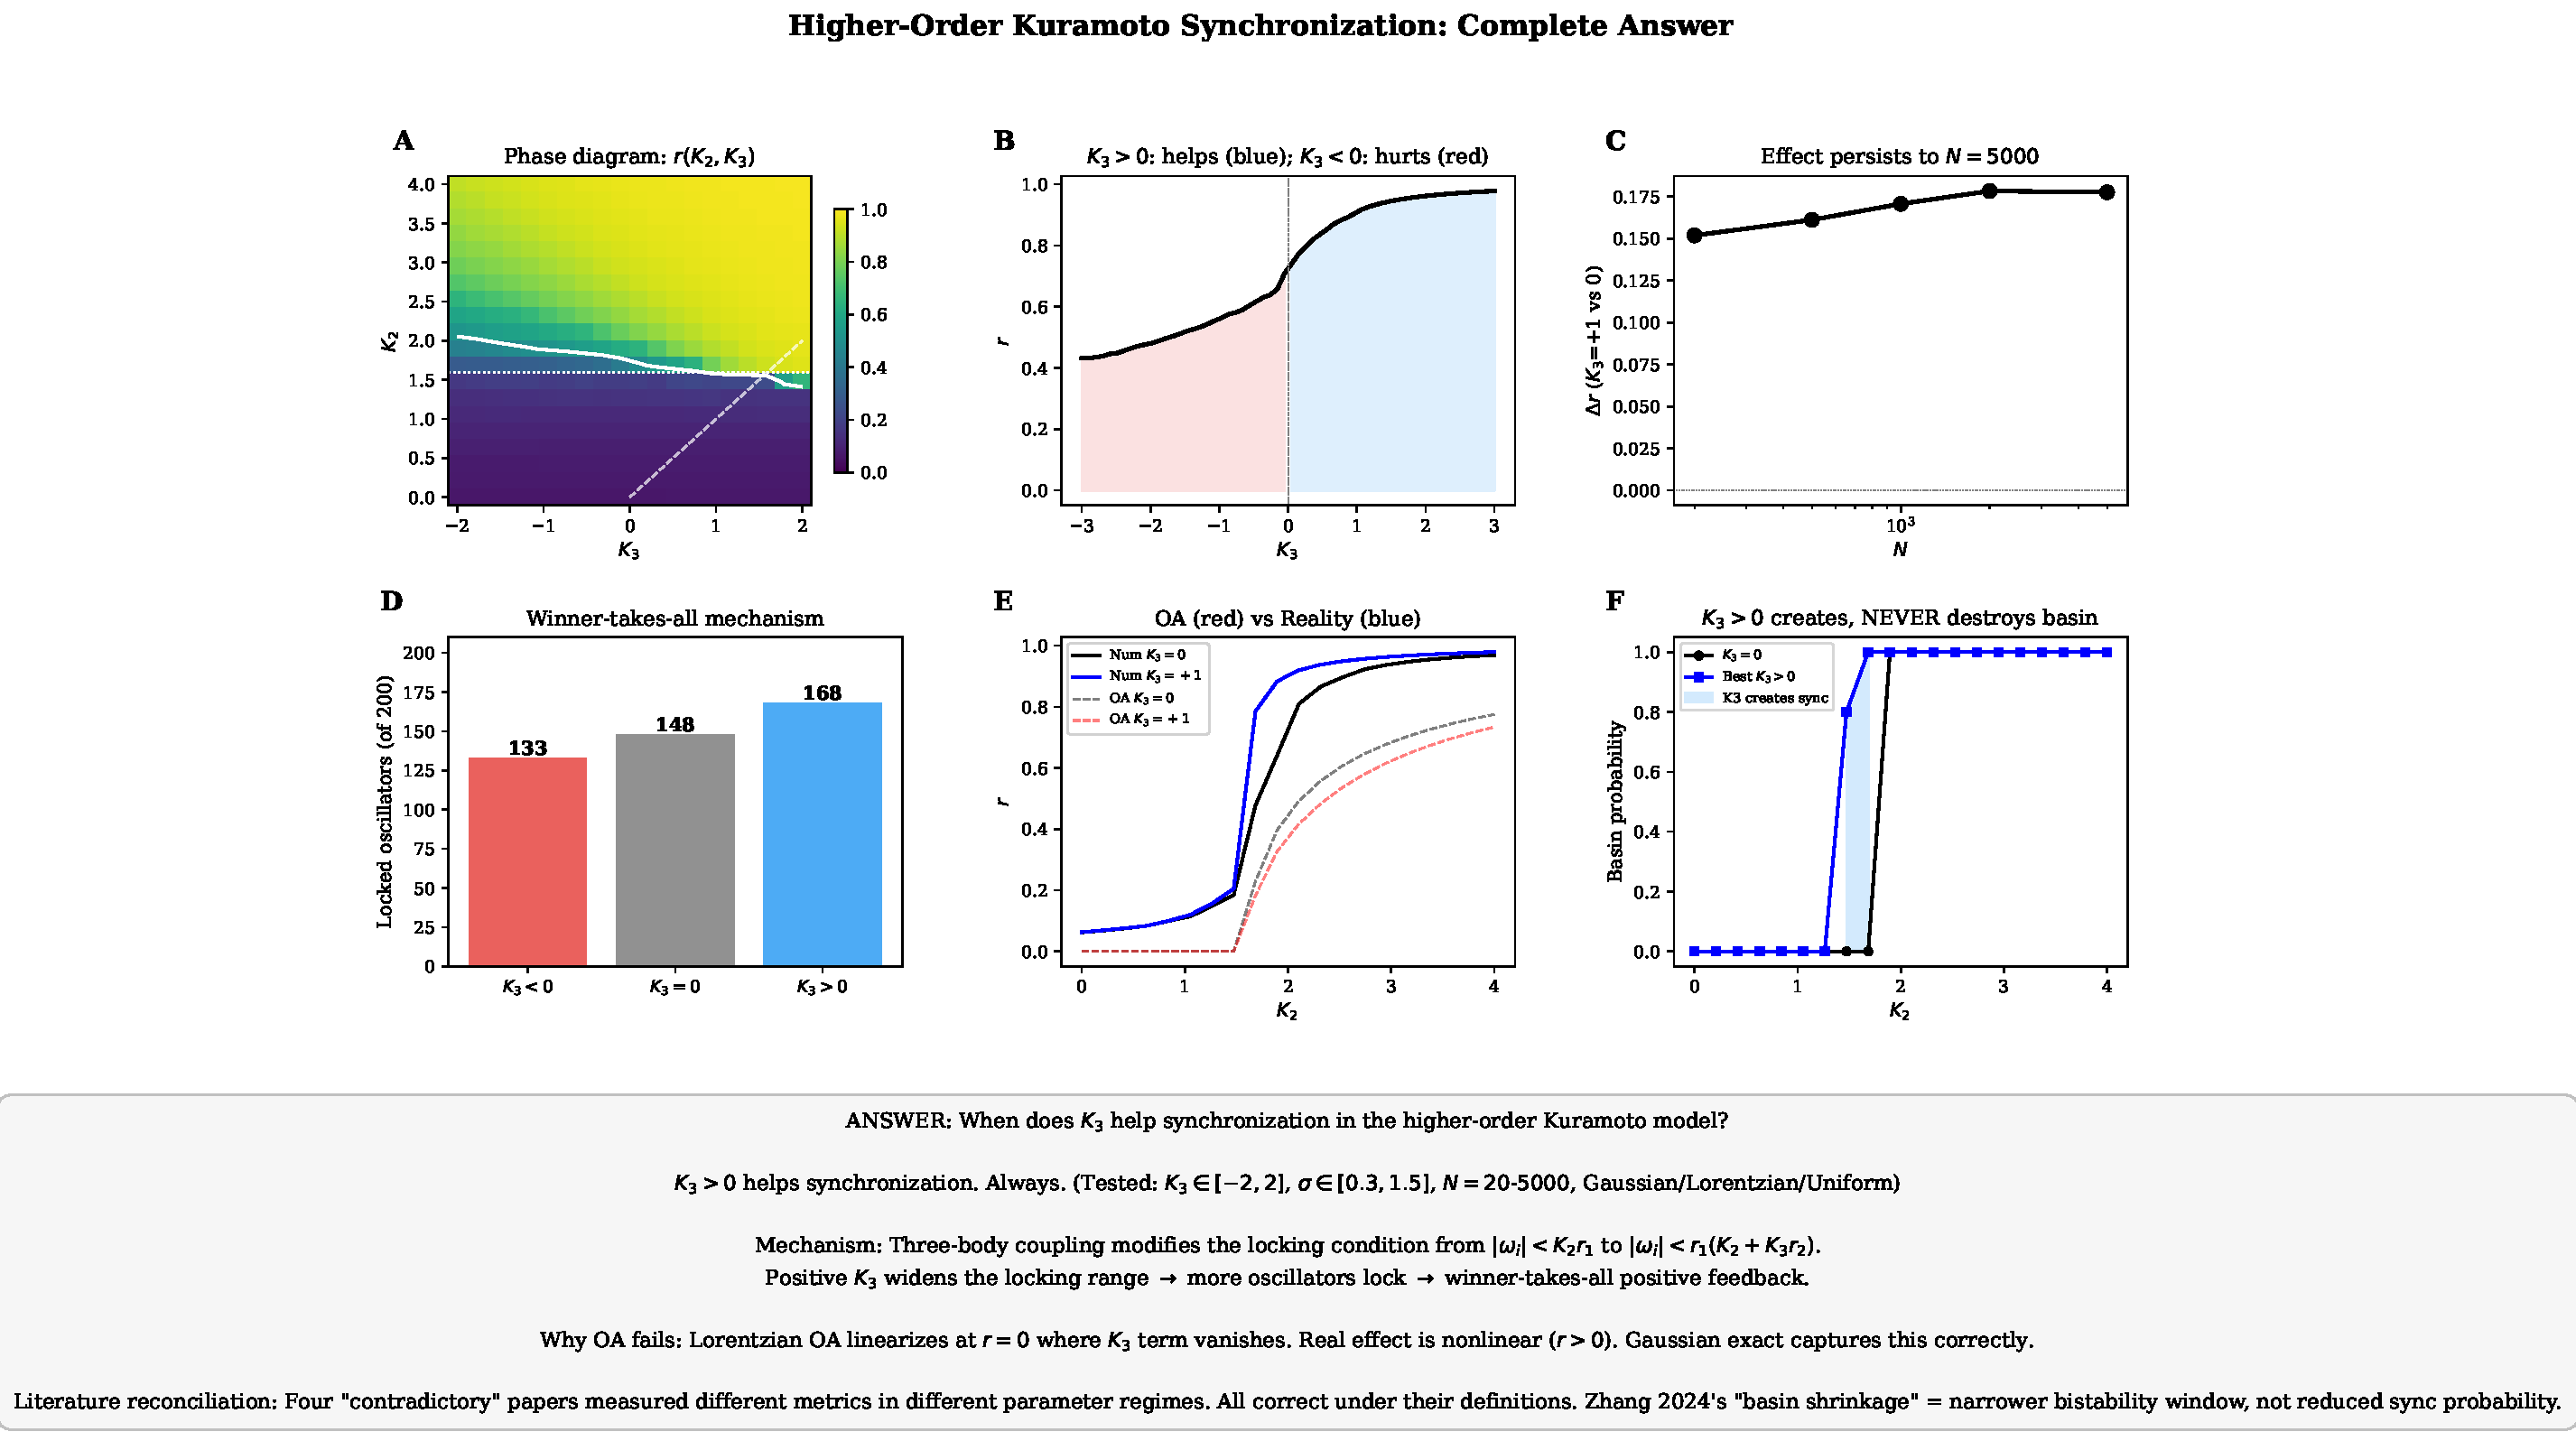
\includegraphics[width=\textwidth]{supplementary/SUMMARY.pdf}
\caption{Visual summary of all key findings.}
\end{figure}

\end{document}
